\section{Experiment}
For each of our experiments we  use the bert-base-uncased BERT model. It has 109m parameters and consists of 12 transformer layers with 768 hidden dimensions, 12 attention heads and a sub word vocabulary of 30,522 tokens. We choose this model because of its success across NLP and question answering, and information retrieval. For ease of reproduction we have build all of our experiments using Hugging Face's Transformers and network pruning was implemented using Neural Magic's sparseml.
\subsection{Question Answering}
For question answering we train using mostly fixed hyperparamets where batch size is 16, learning rate is 3e-5 and we leverage adamW , max sequence length is 384, and all training is done using float16. Models are kept fixed except for train length and any layers that are removed. When we explore removing layers they are removed prior to training and follow the structure described in method. Our baseline matches previously reported results and is achieved in 2 epochs. Our teacher model for distillation is our sparse baseline and after manual experimentation we find a distill hardness of $\lambda=1$ and temperature=2 to be optimal. \\
Our first experiments shown in table \ref{tab:qa-prune-length} show that high sparsity models can retain model performance but training length has to be extended substantially. Our experiments also find that no sparsity is able to support zero shot pruning as this causes huge variations in end model performance (up to 30 absolute F1 percentages). 
\begin{table}[b]
\resizebox{8cm}{!}{
\begin{tabular}{|l|l|l|l|l|l|l|}
\hline
sparsity   & total epochs      & pruned   & one shot   & pruning epochs & F1  & EM\\ \hline
0          & 1                       & no        & no         & 0              & 84.57     & 76.04\\ \hline
0          & 2                       & no        & no         & 0              & 88.02     & 80.63\\ \hline
0          & 10                      & no        & no         & 0              & 87.60     & 79.13\\ \hline
80         & 1                       & yes       & yes        & 0              & 25.14     & 15.10\\ \hline
80         & 2                       & yes       & no         & 0              & 66.96     & 53.88\\ \hline
80         & 10                      & yes       & no         & 8              & 83.95     & 74.41\\ \hline
80         & 30                      & yes       & no         & 18             & 84.06     & 74.64\\ \hline
90         & 1                       & yes       & yes        & 0              & 16.06     & 07.79\\ \hline
90         & 2                       & yes       & no         & 0              & 64.19     & 50.95\\ \hline
90         & 10                      & yes       & no         & 8              & 79.09     & 68.18\\ \hline
90         & 30                      & yes       & no         & 18             & 79.65     & 68.51\\ \hline
95         & 1                       & yes       & yes        & 0              & 10.50     & 04.93\\ \hline
95         & 2                       & yes       & no         & 0              & 24.45     & 14.44\\ \hline
95         & 10                      & yes       & no         & 8              & 72.76     & 60.41\\ \hline
97         & 10                      & yes       & no         & 6              & 70.26     & 57.02\\ \hline
97         & 30                      & yes       & no         & 18             & 70.43   & 57.29\\ \hline
99         & 1                       & yes       & yes        & 0              & 09.69     & 03.61\\ \hline
99         & 2                       & yes       & no         & 0              & 17.43     & 07.87\\ \hline
99         & 10                      & yes       & no         & 8              & 47.31     & 32.56\\ \hline
\end{tabular}}
\caption{Effect of pruning length at various sparsity's for question answering. Short pruning schedules produce irregular results while long pruning schedules produce minor drops in accuracy}
\label{tab:qa-prune-length}
\end{table}
\begin{table}[]
\resizebox{8cm}{!}{
\begin{tabular}{|l|l|l|l|l|l|l|l|}
\hline
sparsity   & params                  & Distilled & pruned   & layers     & pruning epochs & F1 Score   & EM Score  \\ \hline
0          & 108,893,186             & no        & no        & 12         & 0              & 88.00     & 80.63\\ \hline
0          & 108,893,186             & yes       & no        & 12         & 0              & 89.02   & 82.03  \\ \hline
0          & 87,629,570              & no        & no        & 9          & 0              & 86.70   & 78.82  \\ \hline
0          & 87,629,570              & yes       & no        & 9          & 0              & 87.94   & 80.46  \\ \hline
0          & 66,365,954              & no        & no        & 6          & 0              & 81.64   & 72.67  \\ \hline
0          & 66,365,954              & yes       & no        & 6          & 0              & 83.46   & 75.03  \\ \hline
0          & 45,102,338              & no        & no        & 3          & 0              & 51.75   & 39.11  \\ \hline
0          & 45,102,338              & yes       & no        & 3          & 0              & 43.83   & 33.06  \\ \hline
0          & 30,926,594              & no        & no        & 1          & 0              & 26.23   & 17.32  \\ \hline
0          & 30,926,594              & yes       & no        & 1          & 0              & 28.10   & 18.50  \\ \hline
20         & 108,893,186             & no        & yes       & 12         & 18             & 87.20   & 79.17  \\ \hline
20         & 108,893,186             & yes       & yes       & 12         & 18             & 89.56   & 82.74  \\ \hline
40         & 108,893,186             & no        & yes       & 12         & 18             & 86.27   & 78.08  \\ \hline
40         & 108,893,186             & yes       & yes       & 12         & 18             & 89.77   & 83.06  \\ \hline
60         & 108,893,186             & no        & yes       & 12         & 18             & 86.44   & 77.95  \\ \hline
60         & 108,893,186             & yes       & yes       & 12         & 18             & 89.38   & 82.29  \\ \hline
72         & 108,893,186             & no        & yes       & 12         & 18             & 85.50   & 76.43  \\ \hline
72         & 108,893,186             & yes       & yes       & 12         & 18             & 89.11   & 83.04  \\ \hline
80         & 108,893,186            & no        & no        & 12           & 18             & 84.06   & 74.64\\ \hline
80         & 108,893,186            & yes       & yes       & 12           & 18             & 88.03   & 80.81\\ \hline
80         & 66,365,954              & no        & yes       & 6          & 18             & 77.87   & 67.08  \\ \hline
80         & 66,365,954              & yes       & yes       & 6          & 18             & 84.69   & 76.57  \\ \hline
90         & 108,893,186            & no        & no        & 12           & 18             & 79.65   & 68.51\\ \hline
90         & 108,893,186            & yes       & yes       & 12           & 18             & 85.63   & 77.41\\ \hline
90         & 66,365,954              & no        & yes       & 6          & 18             & 73.52   & 61.22  \\ \hline
90         & 66,365,954              & yes       & yes       & 6          & 18             & 80.54   & 71.00  \\ \hline
97         & 108,893,186            & no        & no        & 12           & 18             & 70.43   & 57.29\\ \hline
97         & 108,893,186            & yes       & yes       & 12           & 18             & 75.013   & 63.95\\ \hline
97         & 66,365,954              & no        & yes       & 6          & 18             & 67.27   & 53.86  \\ \hline
97         & 66,365,954              & yes       & yes       & 6          & 18             & 72.36   & 60.82  \\ \hline
\end{tabular}}
\caption{Effect of layer dropping, distillation, and pruning on question answering BERT.}
\label{tab:qa-all}
\end{table}
\begin{figure}[h]
\centering
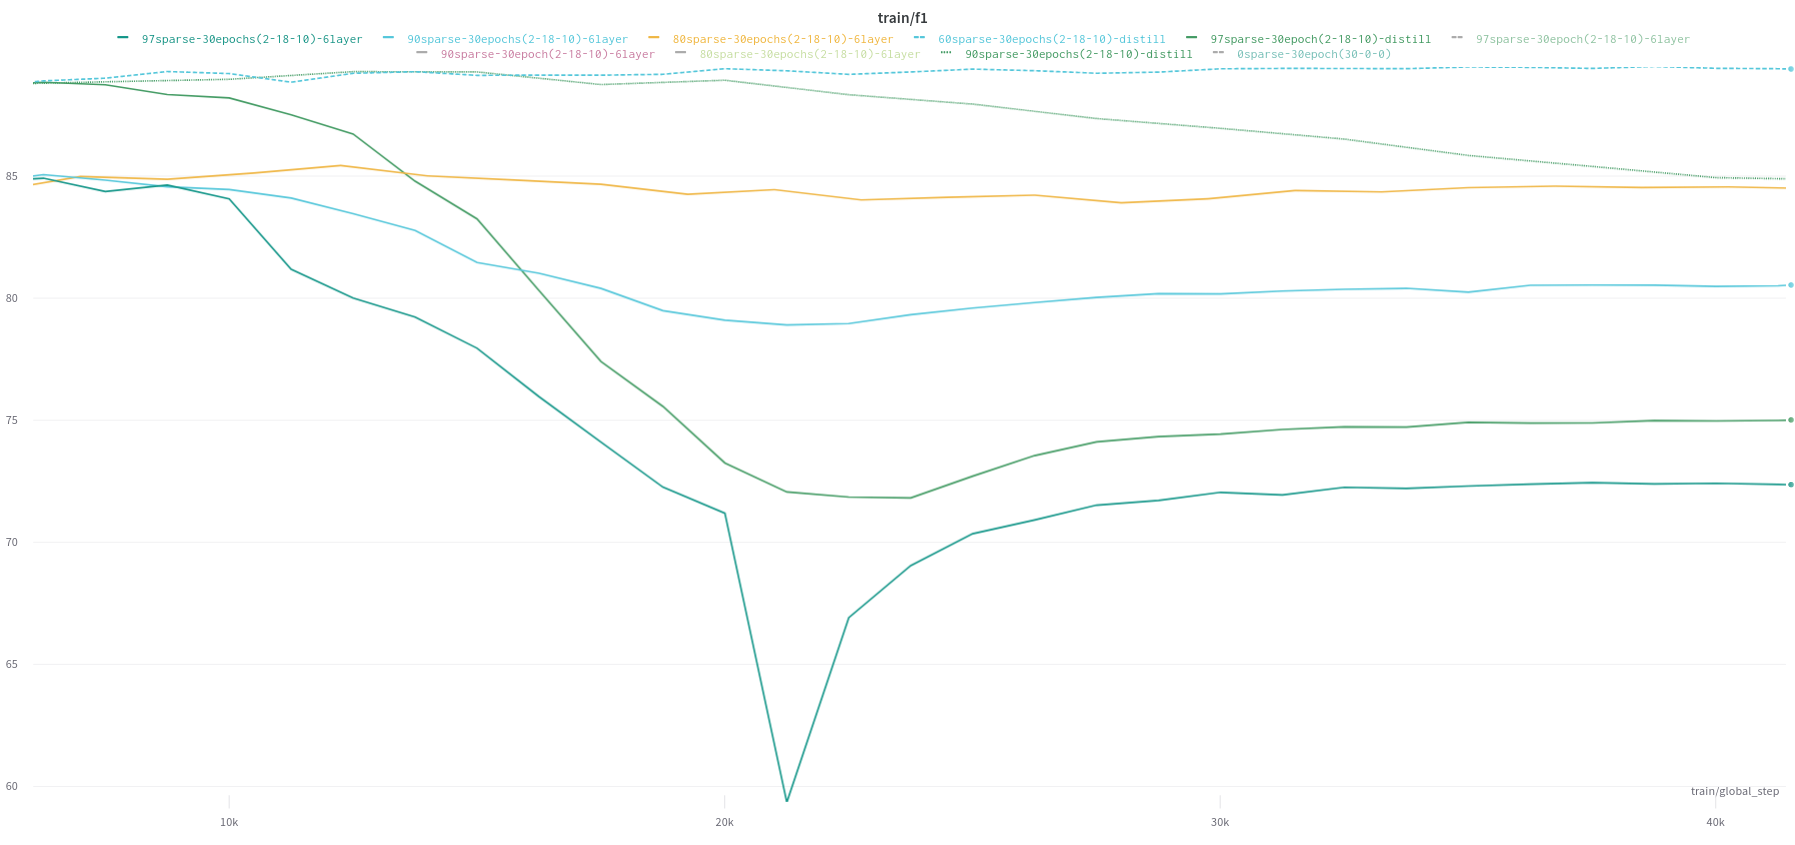
\includegraphics[width=8cm]{project/qaf1.png}
\caption{F1 Variations across question answering compressed models variants over training.}
\end{figure}
\begin{figure}[h]
\centering
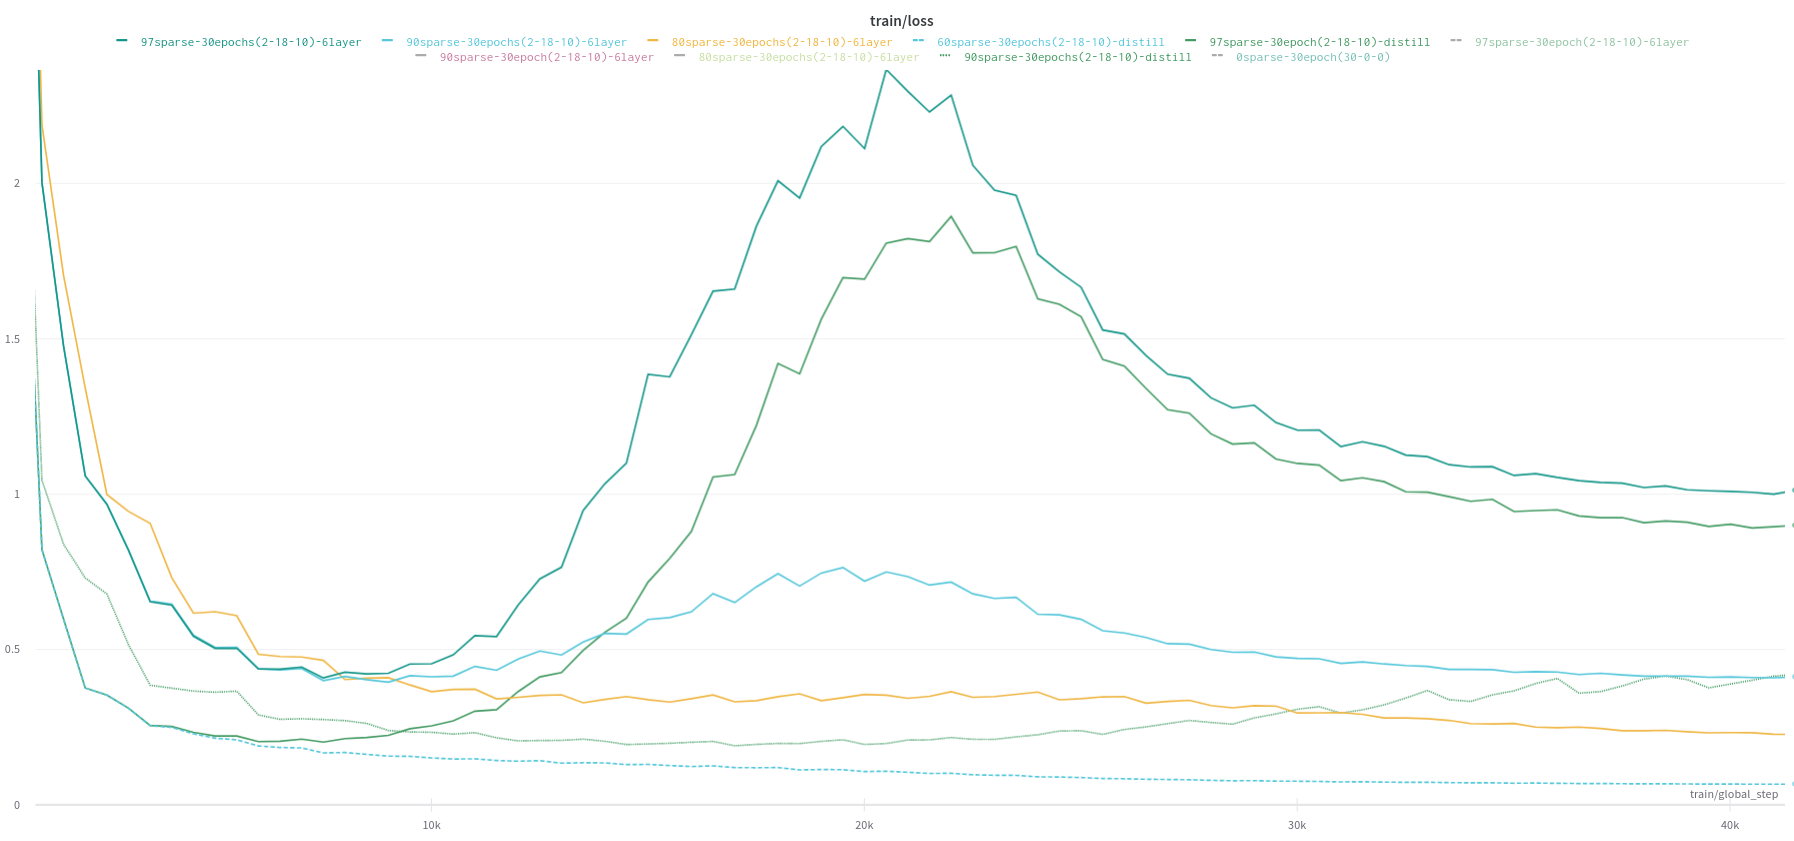
\includegraphics[width=8cm]{project/qaloss.png}
\caption{Loss Variations across question answering compressed models variants over training.}
\end{figure}
Our experiment also find that the relative reduction in parameters caused by layer removal is far more detrimental than network pruning. A distilled model with 72 \% sparsity has about the same amount of parameters as a 3 layer model but its performance is over twice as good and even better than the baseline. We believe this is strong supporter of the effects of sparsity and model distillation as a training regularizer. Our final result show a model with only 2\% active weights only sees a 16 point drop in quality(97\% sparse, 6 layer, distilled) and a 80 sparse, distilled 6 layer model is only 4\% worse than the baseline. On a current state of the art NVIDIA V100 16GB GPU each sample takes 12.77ms \footnote{https://github.com/NVIDIA/DeepLearningExamples/blob/master/TensorFlow/LanguageModeling/BERT/README.md}. When we our sparse models with efficient inference engines like Deepsparse can achieve equal accuracy with 41.19ms/sample on a commodity CPU!
\subsection{Passage Ranking}
Our Approach for passage ranking mirrors our experiments for question answer with minor tweaks to account for the MSMARCO corpus. We update the batch size to 64 and max sequence length to 128. Since the training corpus is ~80m samples, we stop training when loss stops improving. As inference is expensive we do not perform relevance evaluation on each of the 8.8m passages for each query. We use a first stage BM25 model to retrieve and rank the 1000 most relevant pass sage and then re rank those items.  Models are kept fixed except for sparsity, distillation, and layer that are removal. When we explore removing layers they are removed prior to training and follow the structure described in method. \\
As the MSMARCO dataset is over 800,000,000 training examples training on the full dataset is not feasible. Moreover, in long training experiments we do not find any improvement in loss or ranking ability after 1\% of the data is seen. Experiments with distillation found distillation less effective but best results come from a distill hardness of $\lambda=1$ and temperature=2. Experiments with pruning follow findings with our QA pruning experiments and train for 10x as long. It is worth noting that while our re-ranking method outperforms BM25, it does not perform as well as the methods on the MSMARCO leaderboard and are unsure as to why. We experimented with other mixtures of data selection like negative random sampling and negative samples being another positive sample but these dataset provided worse results than the existing MSMARCO dataset. As we could not improve model scores, we focus our efforts on the change with induced sparsity.  \\
The MSMARCO passage ranking dataset has a development set of 6800 queries. For evaluation we follow other work on the dataset and use mean reciprocal rank (MRR) at depth 10 and also study recall at the same depth. For our baseline, we use the public MSMARCO baseline BM25 implementation. As evaluation on this entire dataset takes over 6 hours (6.8 m query url pairs to predict relevance on), we run all of our experiments on a subset of 500 queries as we found that at this size, volatility in metrics is low.\\
Looking at the results shown in table \ref{msmarco} we see that the results are very different than seen in question answering. In passage ranking, model performance does not seem to be heavily tied to model size. Variations in layer removal or pruning rate only have minor degradation's in performance if any. Additionally, unlike question answering, distillation tends to have a negative effect. This is in line with our expectations as the MSMARCO labels are binary and as a result any form of label smoothing is much less important than on probabilities in 384 token context window. Finally, unlike question answering, pruned IR models perform substantially worse despite distillation. It seems that the IR model has learned a ranking function that is more dependent on in layer relations than multi layer transformation. We believe this is interesting because if follows some of the work of other researchers with single layer transformer models. \\
While our results do not point to large differences in performance for compressed passage ranking, we believe this is more of a factor of our model never learning a good representation for the data. Performance for our model is over 30\% worse than some of the other BERT models and as a result model degradation may not be visible as the models have not learned the task well. 
\begin{table}[h]
\resizebox{8cm}{!}{
\begin{tabular}{|l|l|l|l|l|l|}
\hline
sparsity   & distill & layers   & parameters  & MRR@10 & Recall @10\\ \hline
BM25       & no      & N/A      & N/A         & 0.167  & 0.558 \\ \hline 
0          & no      & 12       & 108,893,186 & 0.215  & 0.417 \\ \hline
0          & yes     & 12       & 108,893,186 & 0.213  & 0.427 \\ \hline
0          & no      & 9        & 87,629,570  & 0.208  & 0.397 \\ \hline
0          & no      & 6        & 66,365,954  & 0.208  & 0.397 \\ \hline
0          & no      & 3        & 45,102,338  & 0.207  & 0.395 \\ \hline
0          & no      & 1        & 30,926,594  & 0.207  & 0.395 \\ \hline
80         & no      & 12       & 108,893,186 & 0.199  & 0.403 \\ \hline
80         & yes     & 12       & 108,893,186 & 0.001  & 0.001 \\ \hline
80         & no      & 6        & 66,365,954  & 0.190  & 0.401 \\ \hline
80         & yes     & 6        & 66,365,954  & 0.003  & 0.018 \\ \hline
90         & no      & 12       & 108,893,186 & 0.157  & 0.353 \\ \hline
90         & yes     & 12       & 108,893,186 & 0.001  & 0.002 \\ \hline
90         & no      & 6        & 66,365,954  & 0.179  & 0.367 \\ \hline
90         & yes     & 6        & 66,365,954  & 0.005  & 0.016 \\ \hline
97         & no      & 12       & 108,893,186 & 0.101  & 0.251 \\ \hline
97         & yes     & 12       & 108,893,186 & 0.001  & 0.004 \\ \hline
97         & no      & 6        & 66,365,954  & 0.014  & 0.335 \\ \hline
97         & yes     & 6        & 66,365,954  & 0.003  & 0.016 \\ \hline
\end{tabular}}
\caption{Effect of pruning length at various sparsity's for passage ranking. Removal of layers does not heavily effect performance pruning, distillation and a combination of the three do.}
\label{tab:msmarco}
\end{table}
\begin{figure}[h]
\centering
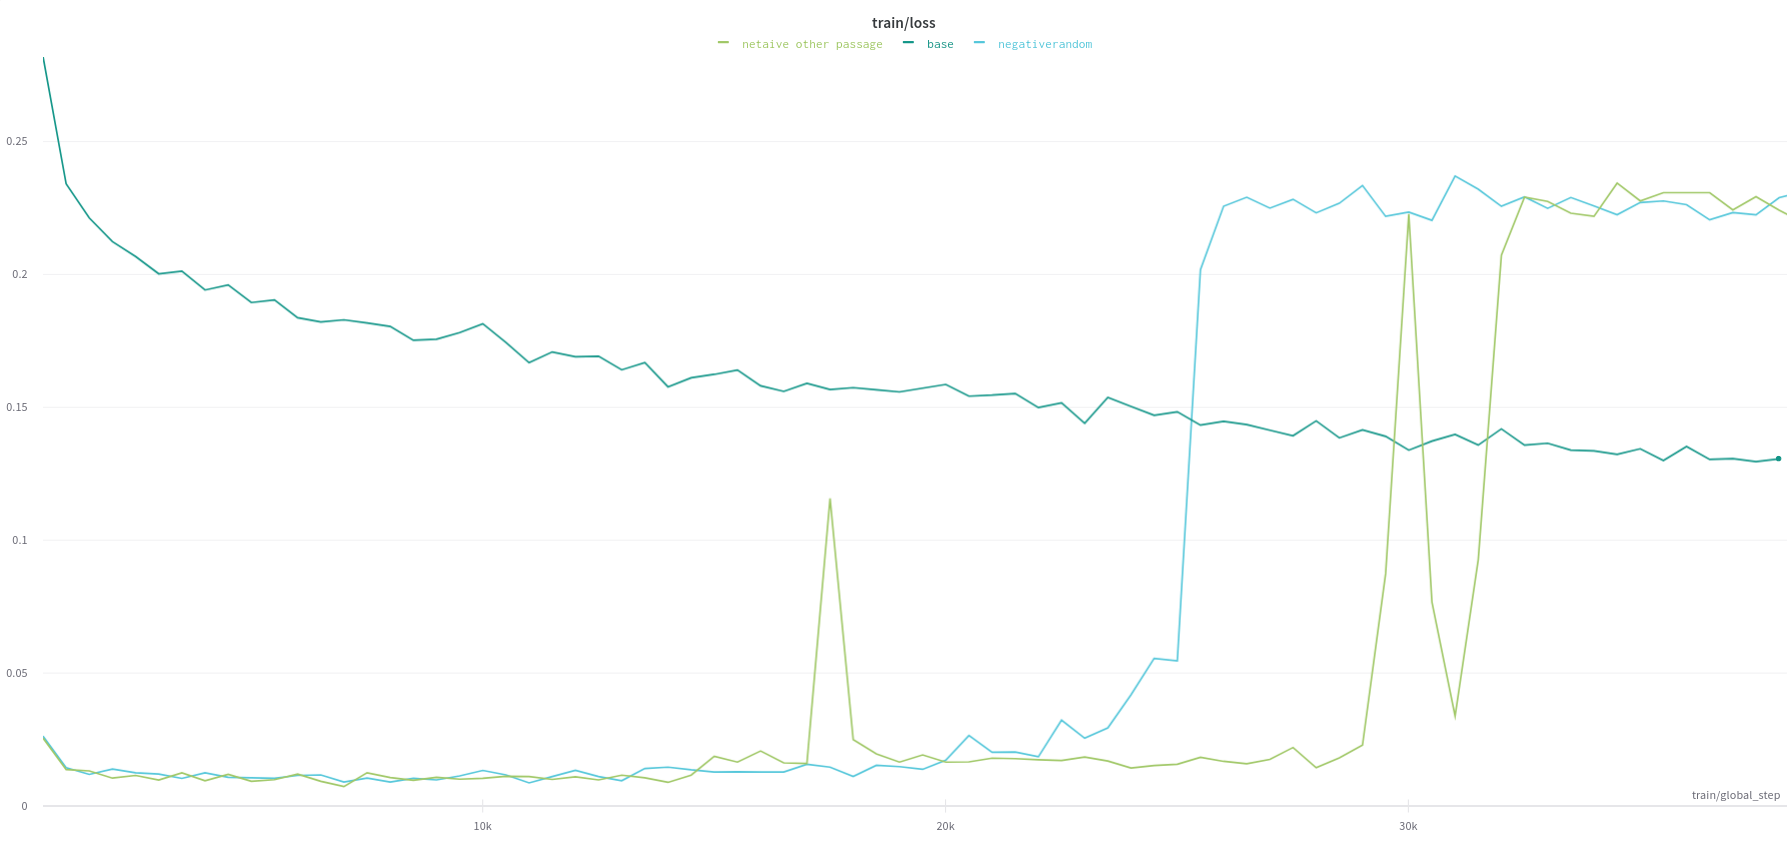
\includegraphics[width=8cm]{project/prunecurves.png}
\caption{Loss Variations across Passage ranking training corpora.}
\end{figure}